\documentclass[tikz,border=10pt]{standalone}
\begin{document}
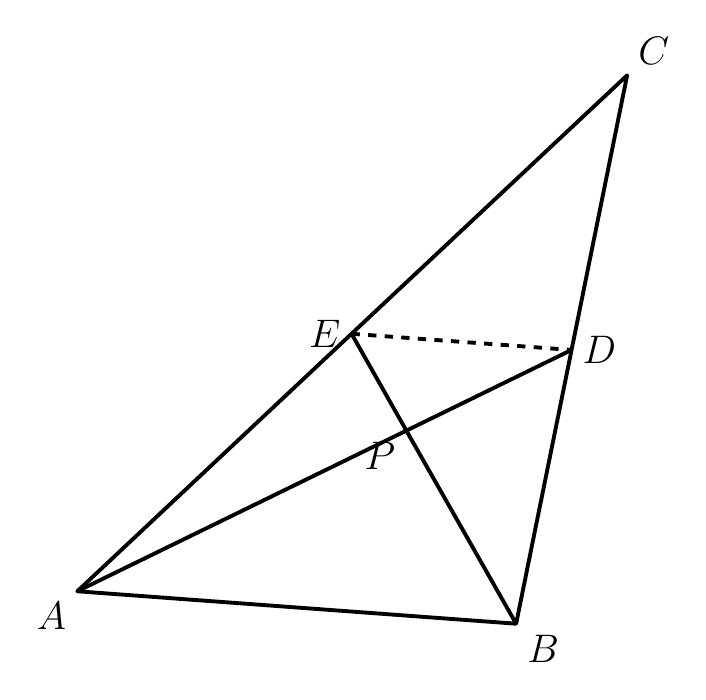
\begin{tikzpicture}[line join=round, line width=1.4pt]
\coordinate (A) at (-3.328,-3.056);
\coordinate (B) at (2.245,-3.468);
\coordinate (C) at (3.655,3.497);
\coordinate (D) at (2.949,0.009);
\coordinate (P) at (0.851,-1.016);



\coordinate (E) at (0.155,0.214);


\draw (A) -- (B) -- (D) -- (C) -- (E) -- (A) -- cycle;


\draw (A) -- (P) -- (D);
\draw (B) -- (P) -- (E);


\draw[dashed] (E) -- (D);


\node[below left, font=\fontsize{14}{16.8}\selectfont] at (A) {$A$};
\node[below right, font=\fontsize{14}{16.8}\selectfont] at (B) {$B$};
\node[above right, font=\fontsize{14}{16.8}\selectfont] at (C) {$C$};
\node[right, font=\fontsize{14}{16.8}\selectfont] at (D) {$D$};
\node[left, font=\fontsize{14}{16.8}\selectfont] at (E) {$E$};
\node[below left, font=\fontsize{14}{16.8}\selectfont] at (P) {$P$};
\end{tikzpicture}
\end{document}